\section{问题二：异构无人机多点多架次调度}

\subsection{模型建立}

在问题一基础上，问题二允许每个架次访问多个服务区并返回 O01，联合确定货箱组批、服务区访问顺序、机型、执行无人机、共享电池与各架次开始时刻。决策变量为：货箱 $c$ 是否由架次 $p$ 运输（$y_{cp}\in\{0,1\}$）、架次 $p$ 的服务区访问顺序 $\sigma_p$、架次 $p$ 的机型选择 $z_{pg}\in\{0,1\}$、开始时刻 $t_p$，以及架次 $p$ 所占用的无人机与共享电池。记 $\mathcal{P}$ 为架次集合、$\mathcal{C}$ 为货箱集合、$\mathcal{B}_g$ 为机型 $g$ 的共享电池池、$g(p)$ 为架次 $p$ 所选机型、$T^{\mathrm{deliver}}_c$ 为货箱 $c$ 的实际交付时刻、$D_c$ 与 $B_c$ 为其医疗期望时刻与首批截止时刻，则可行域由下列七条界定。

\begin{itemize}
	\item[(C1)] \textbf{货箱唯一投送且不可拆：}$\sum_{p\in\mathcal{P}} y_{cp}=1,\ \forall c\in\mathcal{C}$。货箱在架次内不再分包，也不允许同一箱分投两处。
	\item[(C2)] \textbf{载质量与装载体积：}$\sum_{c}m_c\,y_{cp}\le Q_{g(p)}$ 且 $\sum_{c}v_c\,y_{cp}\le V^{\mathrm{load}}_{g(p)}$，$\forall p$。右端是\textbf{架次所选机型}的容量，而机型本身是决策变量，故该约束的右端随 $z_{pg}$ 切换；三个机型的可用装载体积为 $0.06$ / $0.073$ / $0.25$\,m$^3$。
	\item[(C3)] \textbf{返航能量余量：}$E^{T}_p\le\bigl(1-\rho_{g(p)}\bigr)E^{\mathrm{use}}_{g(p)}$，$\forall p$（式~\eqref{eq:energy-margin}）。多区架次的载荷随沿途投送递减，故 $E^{T}_p$ 由逐航段能耗累加得到，而不是按满载全程估算。
	\item[(C4)] \textbf{机型对应的无人机与电池库存：}任一时刻在役的架次数不超过该机型的可用无人机数（全队 8 架，A/B/C 三型各 $4/2/2$ 架），共享电池按机型分池、在役组数不超过池内库存（A/B/C 各 $6/4/4$ 组）。这一条把「机型」与「机队资源」绑在一起，是问题二区别于经典多车场 VRP 的关键：选型不能只看单架次能耗，还要看该型机队是否被别的架次占住。
	\item[(C5)] \textbf{电池充电周转：}每次充电的占用时长按式~\eqref{eq:charging} 的两阶段模型计算，同一组电池的放电占用与充电时段不得重叠；充电占用一并进入资源链传播，即某架次的可用起飞时刻取决于其电池在上一次占用结束后的充电完成时刻。
	\item[(C6)] \textbf{硬时限：}$T^{\mathrm{deliver}}_c\le D_c$（医疗物资）且 $T^{\mathrm{deliver}}_c\le B_c$（首批保障物资），$\forall c\in\mathcal{C}_{\mathrm{med}}\cup\mathcal{C}_{\mathrm{bat}}$。其余货箱的期望送达时刻不进约束，只以加权时延衡量配送及时性。
	\item[(C7)] \textbf{货箱不得跨服务区组批：}$\forall c\in\mathcal{C},\ \forall p:\ y_{cp}=1 \Rightarrow c$ 所在的服务区属于架次 $p$ 的服务区集合，即货箱只与其同一服务区内的货箱并入同一架次，不得跨区拼箱。这一条与问题一的题面约束是同一条，此处并非新增收紧，而是\textbf{求解器已在执行、此前未写进模型}的一条：组批由以服务区为键的数据结构强制（\texttt{code/q2.py} 的 \texttt{merge\_nonurgent} 按服务区归并货箱），货箱在数据结构上无法被换到别的服务区。把它显式列出，问题一与问题二的组批可行域才是同一个。
\end{itemize}

与前期的构造式方案不同，本文把 (C6) 的两类时限处理为\textbf{硬约束}而不是罚项：任一货箱超出其医疗期望时刻或首批截止时刻，该解即判为不可行（目标值取 $+\infty$）并从解空间中剔除，报告前再以断言强制校验硬违约数为 0；只有第三类时限作为软目标进入加权时延 $F_{\mathrm{delay}}=\sum_c w_c L_c$，其中 $L_c=\max(0,\,T_c^{\mathrm{deliver}}-T_c^{\mathrm{expect}})$。这样处理之后，“零违约”就不再是某次运行的幸运结果，而是解空间的定义本身。

优化目标为 $F=w_1 F_{\mathrm{delay}}/R_{\mathrm{delay}}+w_2\,T_{\mathrm{make}}/R_{\mathrm{make}}$，即\textbf{时效优先}：先保证硬时限零违反，再权衡加权时延与全部任务完成时间；架次数与能耗不进入目标，而是作为代价如实报告（处理方式见 6.2 节的 $\varepsilon$-约束）。式中权重取 $w_1=1.0$、$w_2=0.30$，两项各按\textbf{构造基线解自身的取值}归一化，即 $R_{\mathrm{delay}}=\max\{F_{\mathrm{delay}}^{\text{基线}},\,1\}$、$R_{\mathrm{make}}=\max\{T_{\mathrm{make}}^{\text{基线}},\,1\}$。这样取是因为时延以秒计、完工时间亦以秒计，二者量级相近却\textbf{不同源}：用各自的基线值作标度，权重才表达“单位相对改进”的交换比，而不是被量纲差掩盖。以构造基线为标度的另一个好处是权重不必随算例规模重新标定——基线本身就是同一算例的参考水平。$w_2/w_1=0.30$ 表示\textbf{一比一权衡下}，宁可多等 1 单位相对时延以换取 0.3 单位相对完工时间。这里必须讲清楚一件事：按基线值归一化后，两项的边际交换比被固定为 $0.30\,R_{\mathrm{delay}}/R_{\mathrm{make}}$，在本算例的基线上折算下来是“1\,s 完工抵十余秒时延”——\textbf{这与题面「及时性优先、其次完工、最后能耗与架次」的次序并不一致}。故本文对 $F$ 的定位是\textbf{搜索的下坡方向}，而不是最终取舍：$F$ 提供的平滑梯度用于让 ALNS 稳定收敛，\textbf{最终择档改用题目优先级的字典序}（式~\eqref{eq:q2-key}），两把尺子的分工见 6.2 节第 (6) 条。此外，$\varepsilon$-约束扫描时对超出架次数上界 $\varepsilon$ 的部分施加线性罚 $0.50\,(\text{架次}-\varepsilon)$，用于把搜索压回该档的可行域，档内最终解仍须满足架次数 $\le\varepsilon$ 并复检（见 6.2 节）。

\subsection{求解策略}

鉴于问题规模与约束耦合，本文采用“构造基线 + 大邻域自适应搜索（ALNS）+ $\varepsilon$-约束扫描”的求解框架，并另做两层小规模精确验证。

\textbf{（1）求解框架与精确组批初始解。}本文的求解链为“精确组批 $\to$ 路线全排列精化 $\to$ 瓶颈感知解码 $\to$ ALNS 破坏—修复搜索 $\to$ $\varepsilon$-约束逐档扫描 $\to$ 逐档定型 $\to$ 按题目优先级择档”，如图~\ref{fig:q2-algorithm}所示。初始架次集合不再由贪心规则给出，而是对每个服务区做一次\textbf{精确装箱}：先枚举该区非紧急货箱的全部“载质量—体积”可行子集，再用子集 DP（状态压缩）求字典序（批次数 $\to$ 能耗和 $\to$ 时间和）最优的划分；候选池由 A/B/C 三型各自的可行子集按货箱掩码合并去重、逐掩码保留机队代价最优的机型构成，于是重载子集自然由 C 型承载，轻载子集则可能由 A/B 型以更低能耗承载。紧急货箱（医疗与首批）仍按“每区单独成架次”构造——这条是硬时限的保证，不交给搜索去试探。区箱数超过 16 或存在单箱超限时回退 FFD，以免子集枚举规模失控。该初始解只作为搜索起点，其质量由 6.4 节的精确解标定。

这里须交代一处实现口径，它关系到「表里的解」与「落盘的解」是不是同一个：\textbf{搜索内核}（破坏—修复主循环、可行档案与接受准则）沿用本文 \texttt{code/q2.py} 的 \texttt{alns}，v2 引擎替换的是它的三层外围——\textbf{构造层}（精确组批取代 FFD 构造）、\textbf{解码层}（\texttt{q2.schedule(dispatch="balanced")}，把选型记账统一到一处）、\textbf{派工择序层}（插入式局部寻优与退火搜索），并加上多种子与档间热启动；逐档解在落盘前还要过 7.4 节的中继门禁重排。只换外围而不换内核，是因为内核的接受准则与可行档案决定了「搜索途中路过的可行好解不会被丢掉」这一性质；外部实现把这两条改成「不可行解一律不接受、只留末端最优」，本文\textbf{没有}移植，否则会凭空损失可行解。

% 画布 816×384 px，横版三栏（宽高比 2.13），与图 2.1《总技术路线图》同宽同字号；
% 按 \textwidth 插入后图内文字约 9.5 pt。源文件由 code/make_q2_algorithm.py 生成。
\begin{figure}[htbp]
	\centering
	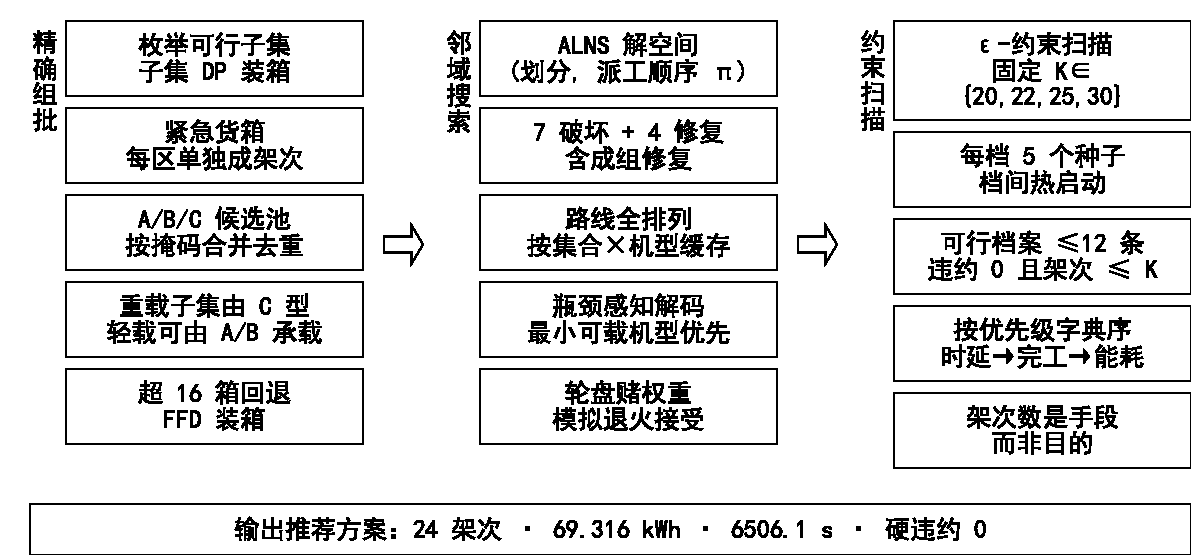
\includegraphics[width=\textwidth]{figures/fig_q2_algorithm.pdf}
	\caption{问题二求解框架}
	\label{fig:q2-algorithm}
\end{figure}

\textbf{（2）路线全排列与瓶颈感知解码。}给定一架次所服务的服务区集合，其访问顺序仍有 $k!$ 种可能；服务区数不超过 5 时（$5!=120$）本文对全部排列精确枚举，硬时限箱以最早交付为平局键，结果按“服务区集合 $\times$ 机型”缓存复用。解码（把架次集合落成“哪架无人机、哪组电池、几点起飞”）同样不是逐架次贪心：调度函数 ${\rm schedule}(d,\mathcal{T},\pi)$ 接受一个派工优先级排列 $\pi$ 并做\textbf{瓶颈感知选型}——在 $\pi$ 给定的次序下，候选机型的评分为「开始时刻 $+300\times$ 机型重载序」（A/B/C 记 $0/1/2$），即在 $300$\,s 的让位窗口内优先把架次派给\textbf{装得下的最小}机型，同分再比能耗。这一项之所以必要，是因为“能耗最小”的机型未必是机队瓶颈所在：C 型每箱公里最省电，若一味按能耗选型，总时长会堆到只占机队四分之一的 2 架 C 型机上，完工时刻被该机型的串行时长钉死，而与总工作量无关。仅改变 $\pi$ 就会改变无人机与电池的可用时刻，进而同时改变架次数、能耗与完成时间三个指标——实测把 $\pi$ 由“紧迫度升序”换成“最早完成时刻优先”即可使完成时间下降约 $2\%$。故本文的解空间定义为 $(\text{货箱}\to\text{架次的划分},\ \pi)$ 二元组。

\textbf{（3）ALNS 的破坏与修复算子。}在上述解空间上实施自适应大邻域搜索\cite{pisinger2007general}，共 \textbf{7 个破坏算子}：随机移箱、Shaw 相关移箱（按时空邻近性成簇摘除）、最差架次整体拆除、按服务区整体移除、仅移除非紧急货箱、整架次拆解、以及仅扰动顺序而不动划分；配 \textbf{4 个修复算子}：贪婪插入、Regret-2 插入、新开架次、以及成组修复。算子权重按轮盘赌自适应更新（段长 100 次迭代、平滑系数 $\rho=0.25$），接受准则采用归一化目标上的几何降温模拟退火。其中“成组修复”是为解决下述代理代价缺陷而专门加入的：贪婪插入用“该架次最省机型代价”作为插入位置的代理代价，而该代理假设每架次可自由选用最省机型，\textbf{看不到机队资源竞争}，会系统性地漏掉“并区以腾出紧缺机型”这类协同动作。成组修复改为对候选前 $10$ 个位置做真实解码评估，代价更高但能看见资源竞争。

上述破坏—修复算子、$\varepsilon$-约束逐档扫描与消融对照的实测表现汇总于图~\ref{fig:q2-alns}，该图并排给出收敛轨迹、消融比值与四档非支配关系三张诊断。

% 图片宽度 10.0 in，按 0.95\textwidth=6.17 in 插入，缩放比 0.617
\begin{figure}[htbp]
	\centering
	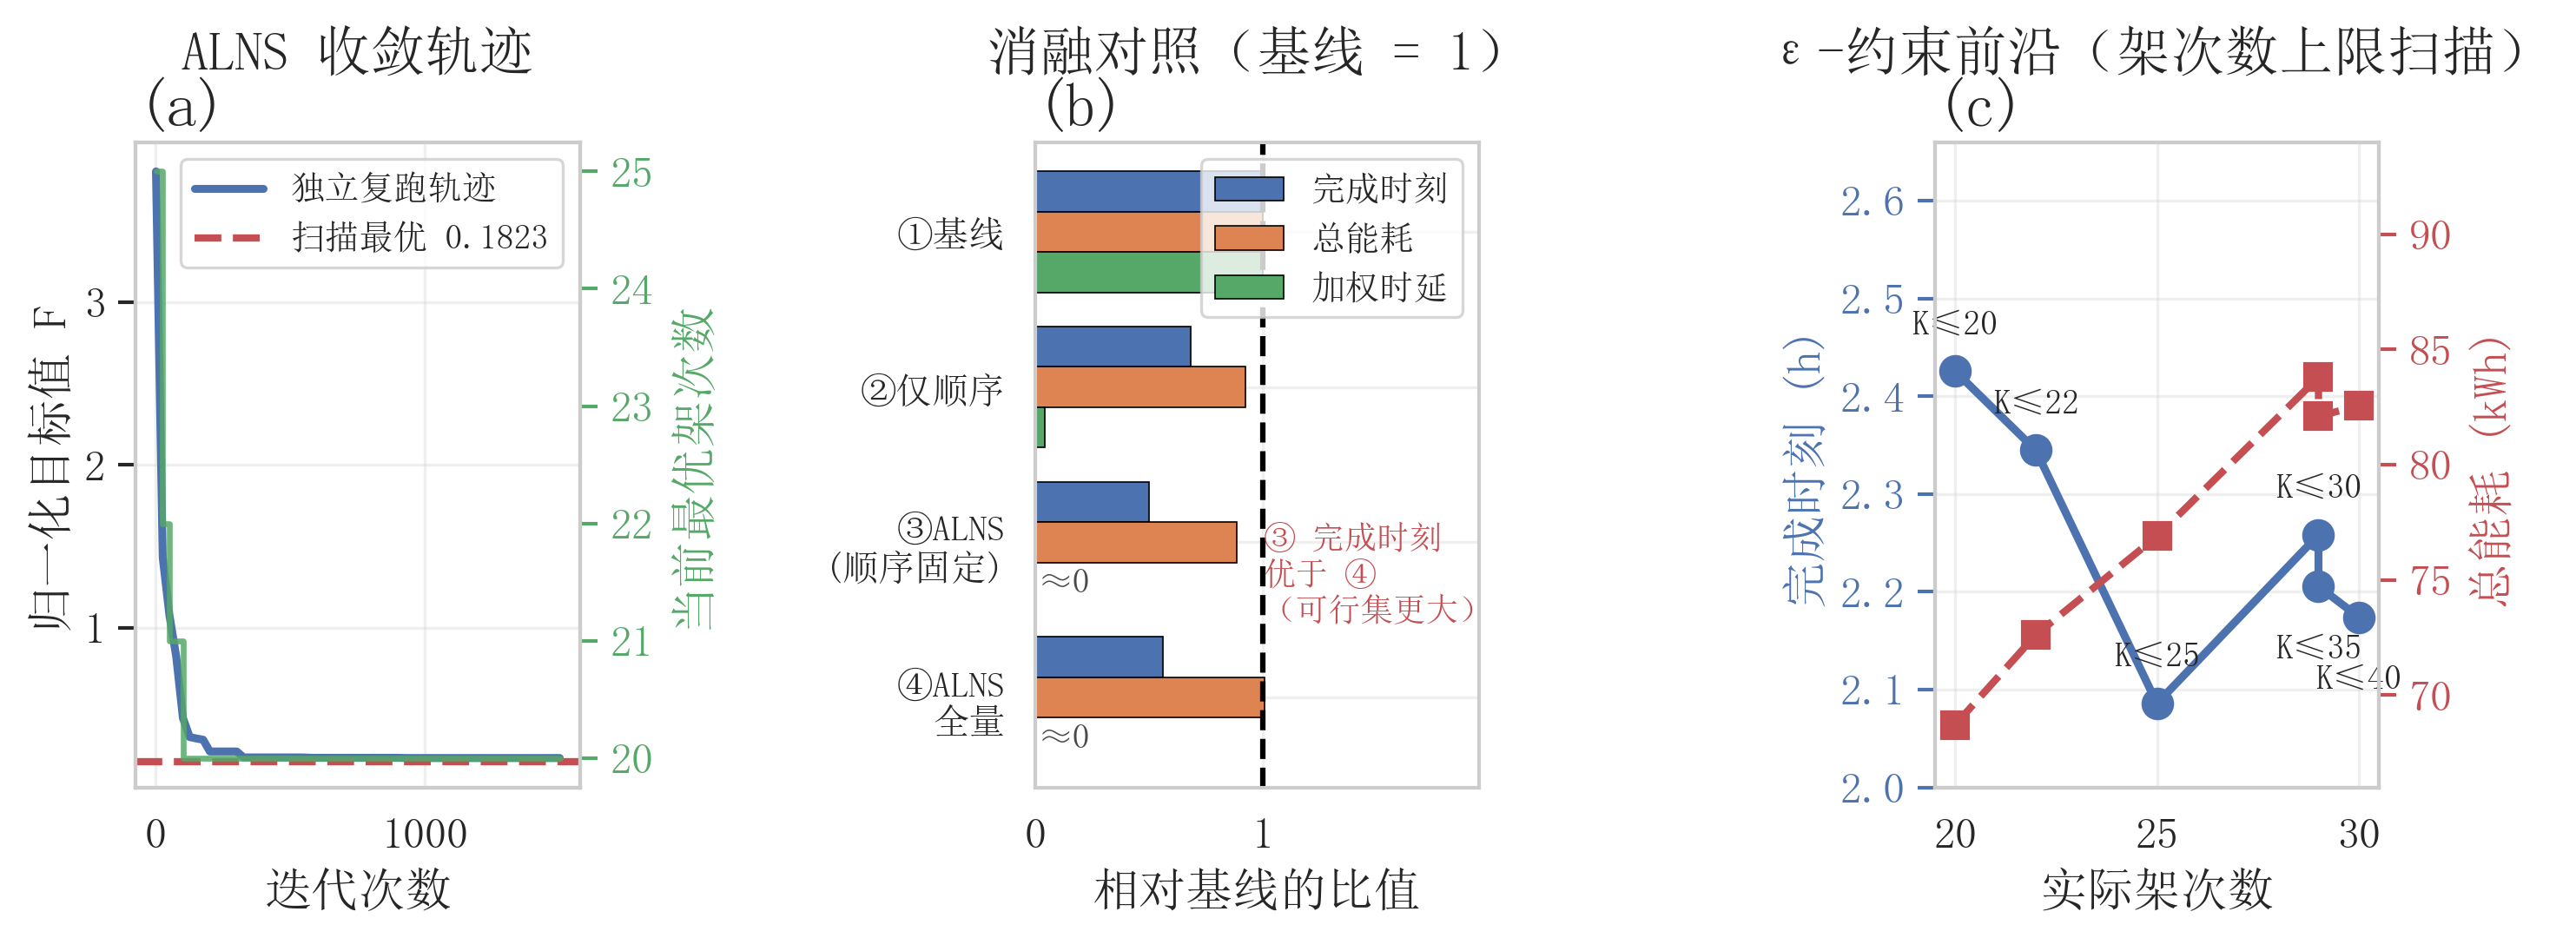
\includegraphics[width=0.95\textwidth]{figures/fig_q2_alns.png}
	\caption{ALNS 收敛、消融对照与 $\varepsilon$-约束扫描}
	\label{fig:q2-alns}
\end{figure}

图~\ref{fig:q2-alns}给出搜索过程的三项诊断：(a) 推荐档（$K\le25$）\textbf{那一次真实运行}的目标值收敛曲线（每 $58$ 次迭代记一点的抽样记录），其终值 $0.145602$ 与表~\ref{tab:q2-pareto}中 $K\le25$ 档的目标值一致，即曲线确为所求方案本身的轨迹；实测全部 $4$ 次改进都发生在第 $465$ 次迭代之前，此后连续 $1\,500$ 轮档案无改进、触发耐心早停，该档于第 $1\,973$ 次迭代终止（故轨迹短于 $3\,500$ 轮的预算上限，这是早停而非记录缺失）——可见预算的绝大部分用于确认而非改进；(b) 表~\ref{tab:q2-ablation}五项消融的并排对照，三项指标一律化成\textbf{相对基线①的比值}才画得进同一张图（量纲相差几个数量级）——除④的总能耗高于基线（比值 $1.054$）外，其余各项都落在 $1.0$ 左侧，③的加权时延被压到 $0$ 故在柱位上就地标出「$\approx 0$」，读者一眼可看出“顺序”与“组批”各自解决了什么；(c) 四个档位的架次数—能耗—完成时间扫描，其中\textbf{实心点}连线的是四维非支配档，\textbf{空心点}为被支配档——被支配关系连同各档指标一并列于表~\ref{tab:q2-pareto}，读者可逐档核对。

\textbf{（4）$\varepsilon$-约束逐档扫描。}架次数是手段而非目的，且与时延、完成时间直接对抗，故不把它与时延平权加权，而是取为约束逐档扫描：固定架次数上限 $K\in\{20,22,25,30\}$，在各档内最优化时效目标。这里 $K$ 是\textbf{货真价实的约束}：搜索中间态允许暂时超出 $K$，以便破坏算子拆散架次后重新合并，但每一档的候选解只从“硬违约数为 $0$ 且实际架次数 $\le K$”的\textbf{可行档案}中录取，导出前再复检一次；某档若全程未找到可行解，则如实记为该档无解，不以超 $K$ 的方案顶替。每档独立运行 5 个随机种子（种子取 $20260923+101K+7919s$，互不重叠），并把上一档的最优解热启动进下一档；档案按（架次、完成时间、能耗、时延）去重，上限 12 条。

档位上限为什么收到 30 而不更大：\textbf{通信连续性是问题三的硬约束}，而需要同时护航的运输架次会随架次数上升。这一收窄来自上一轮更宽扫描（六档，原始记录见 \texttt{\_legacy/q2\_v1/q2\_pareto.csv}）的实测：$K\le35$ 与 $K\le40$ 两档的完成时间更短，但其并发中继需求峰值达 3，已超过题给的 2 架中继无人机，问题三只能以中断收场。故本文把档位收窄到 $K\in\{20,22,25,30\}$——即扫描过的六档中“问题三可零中断”的那四档——再在其中择档，否则会出现“问题二指标更优、整卷方案却违反硬约束”的自相矛盾。需要说清的是：本轮只重跑了收窄后的四档，宽档的两条记录是上一轮同口径扫描的结果，作为问题二—问题三耦合的实测证据在 7.6 节引用，本文不把它表述为“已证明 $K\le35$ 必然中断”。

\textbf{（5）逐档定型轮。}档案里的解是搜索途中的快照，其派工顺序未必已经收敛。故对\textbf{每一档}的代表解再跑一轮定型：先做派工顺序的插入式局部寻优（架次集合不变，接受准则为完成时间、能耗、加权时延三项的严格 Pareto 改进，故不可能变差），再做一轮退火派发顺序搜索，用于消掉“必须让中间态先变差才腾得出来的尾部”。两轮都只动 $\pi$，路线与架次数不变，$K$ 档约束仍成立。之所以逐档都做、而不是只做最终被选中的那一档，是因为交付的推荐方案就是其中一档：若各档定型程度不一，档间比较就失去可比性，而且“表里那一行”与“落盘的方案”就不再是同一个解。

\textbf{（6）择档键按题目优先级字典序。}搜索使用的标量目标 $F$ 把加权时延与完成时间按 $w_1\!:\!w_2$ 折算，用于给搜索提供平滑的下降方向；但\textbf{折算本身会引入交换比}——两项参考量相差一个量级，等价的边际权重并不符合题目给定的“及时性优先、其次完工、最后能耗与架次”次序。故\textbf{终选不沿用 $F$}，而是按题目优先级逐层比较
\begin{equation}
	\text{key}=\bigl(\ \text{加权时延},\ \text{完成时间},\ \text{总能耗},\ \text{架次数},\ K\ \bigr),
	\label{eq:q2-key}
\end{equation}
前一层严格更优即定胜负；同层内相差小于 $10^{-6}$ 视为并列（不让浮点噪声决定胜负），继续比下一层。两把尺子分工明确：$F$ 管搜索方向，式~\eqref{eq:q2-key} 管最终取舍；逐档定型的代表解在式~\eqref{eq:q2-key} 下最优者即为推荐方案。本问的求解规模为：80 个货箱、8 架无人机、14 组共享电池，解空间是「80 箱到架次的划分 $\times$ 派工排列 $\pi$」的二元组；单次搜索 3\,500 轮迭代、7 个破坏算子与 4 个修复算子，$\varepsilon$-约束取 $K\in\{20,22,25,30\}$ 四档、每档 5 个种子，合计 20 次独立搜索；精确验证两层中，分区层为集合划分整数规划、时序层为 big-$M$ 析取 MILP，算例规模见 6.4 节。

\subsection{求解结果}

按式~\eqref{eq:q2-key}的题目优先级字典序，本文取 $K\le25$ 一档作为推荐方案：共 \textbf{24 个运输架次}，全部 80 个货箱在硬时限内完成交付（医疗期望与首批保障违约数均为 $0$，加权时延为 $0$），总运输能耗 $69.316$\,kWh，全部任务完成时间 $6506.1$\,s（$1.81$\,h）。资源使用情况为：8 架实体无人机全部投入使用，14 组共享电池参与周转（A/B/C 型分别为 6/4/4 组），与库存完全一致，满足资源可行性。24 个架次中有 3 个访问两个服务区（T08: S010$\to$S014、T12: S001$\to$S010、T21: S011$\to$S008），正是这几条跨区架次把 15 个服务区绑定为问题四所需的原子任务单元（见 8.1 节）。调度甘特图如图~\ref{fig:q2-gantt}所示。

\begin{figure}[htbp]
	\centering
	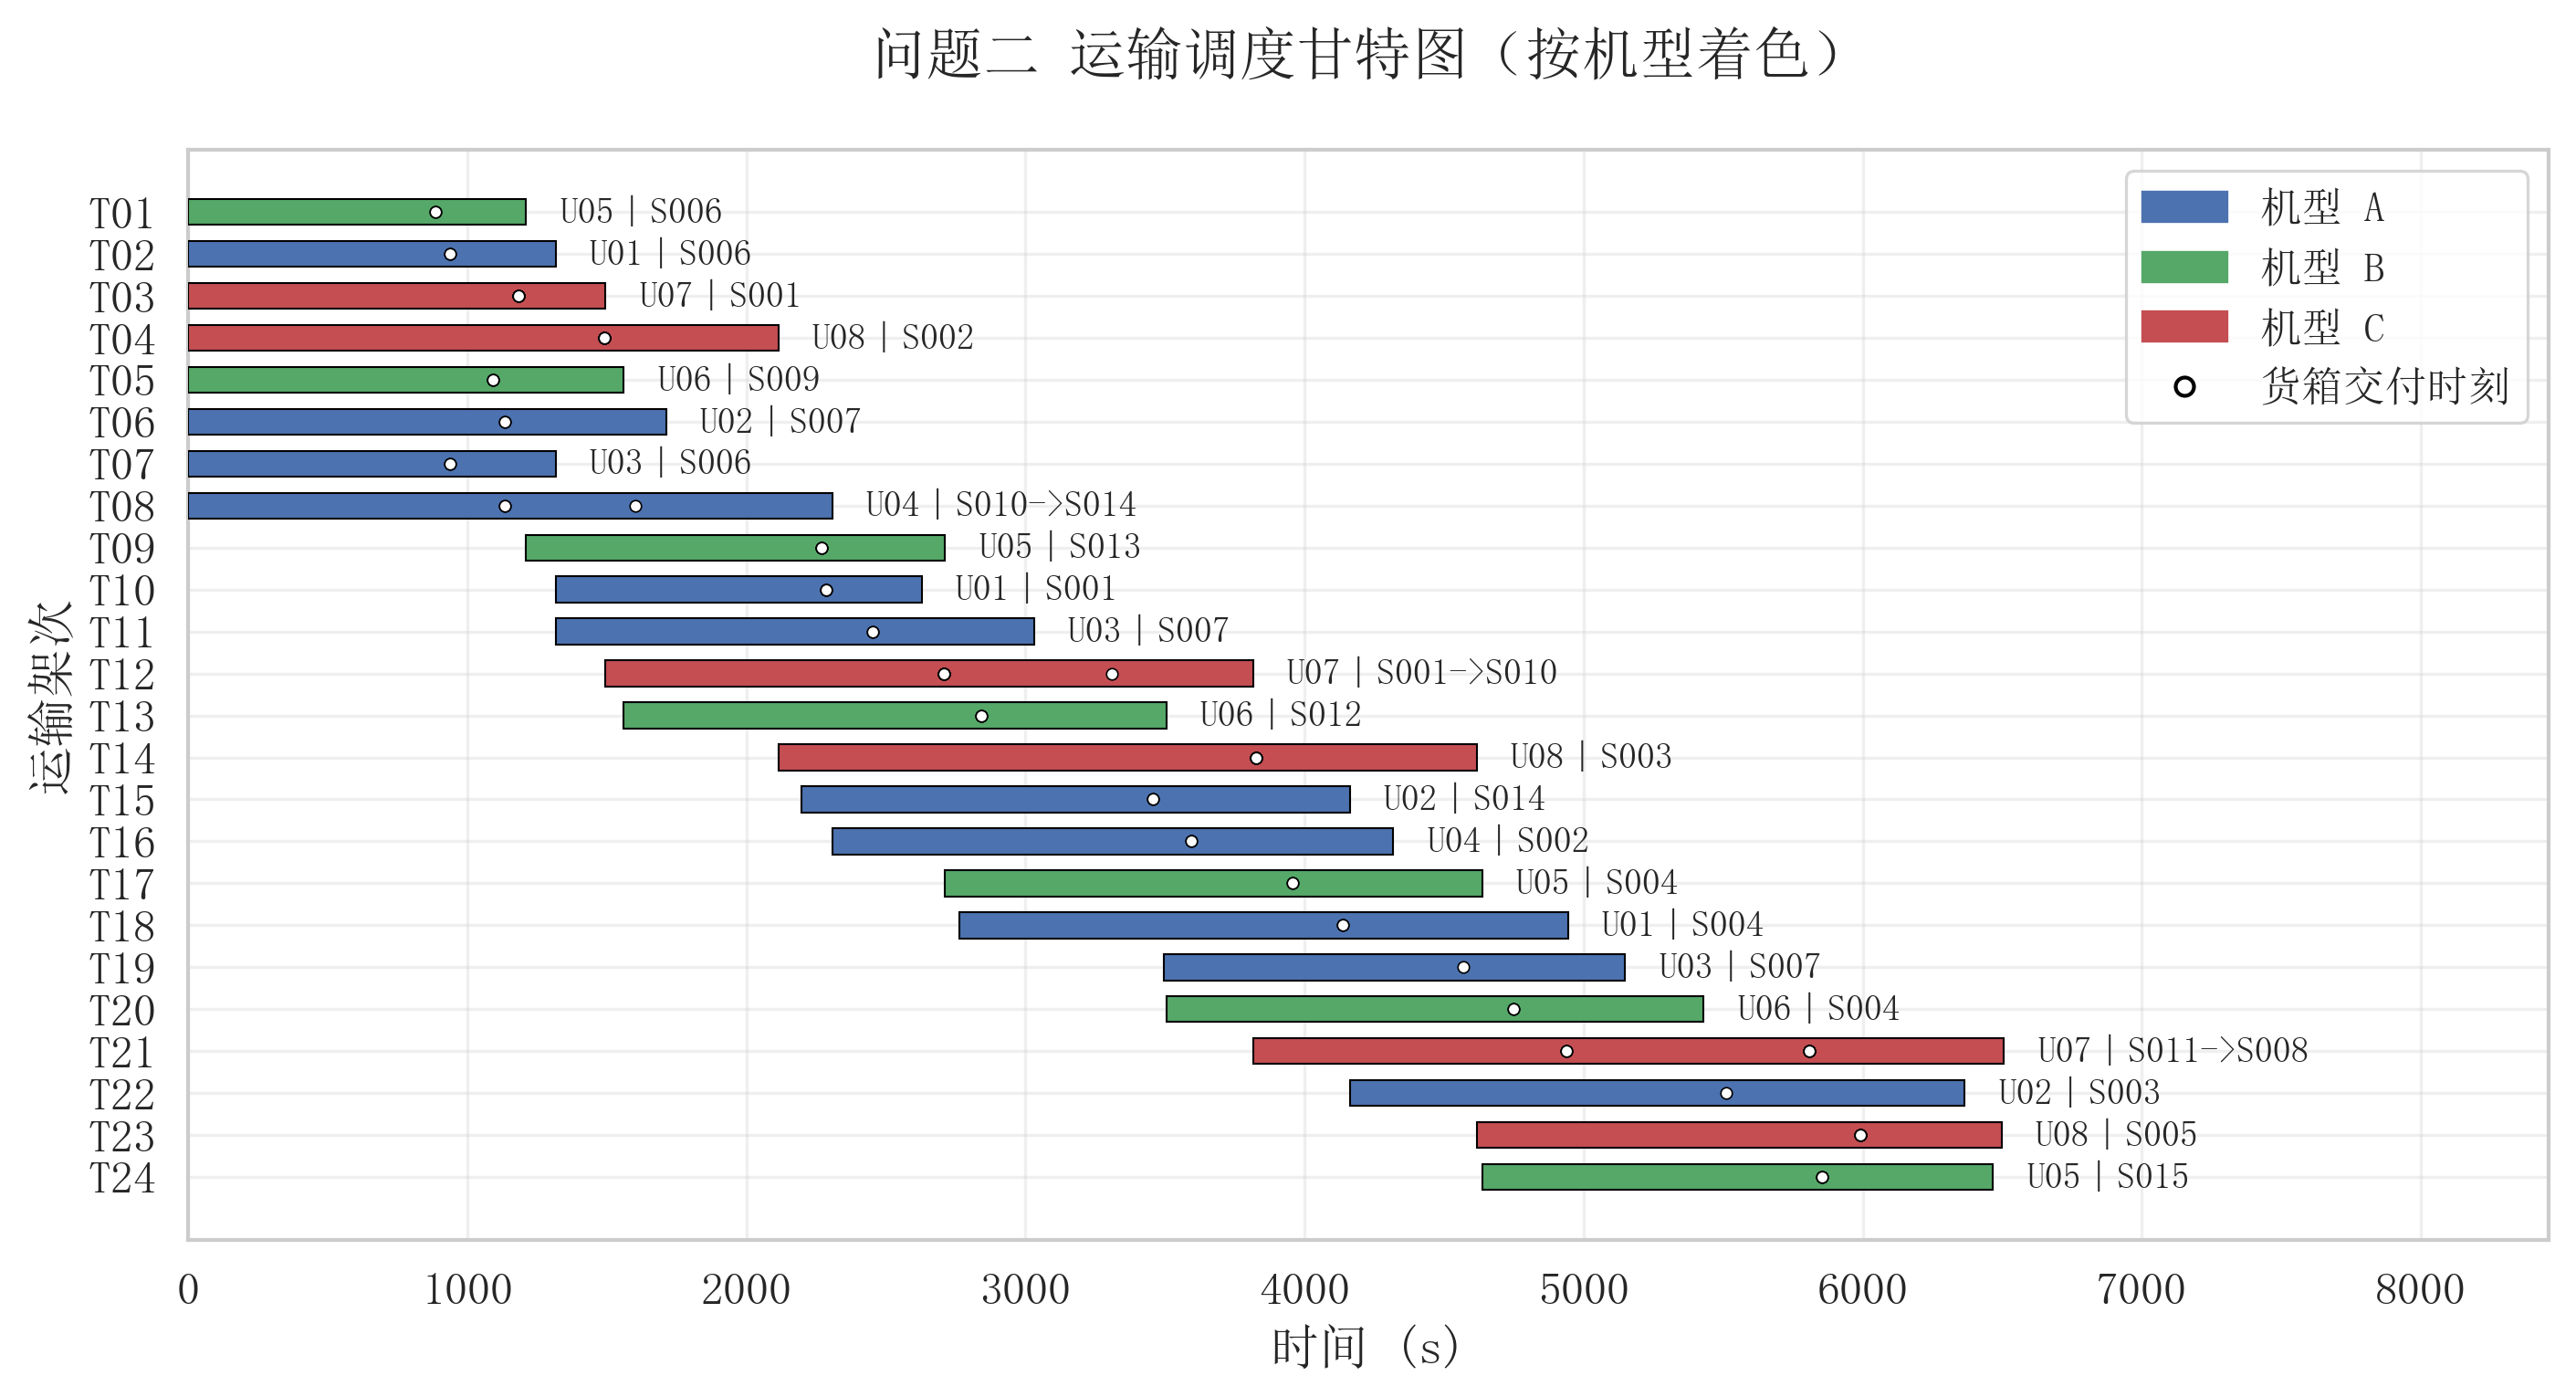
\includegraphics[width=0.92\textwidth]{figures/fig_q2_gantt.png}
	\caption{问题二推荐方案运输调度甘特图}
	\label{fig:q2-gantt}
\end{figure}

图~\ref{fig:q2-gantt}把 24 个架次按机型铺在一条共享时间轴上，横轴刻度即任务时钟，条右端的空心圆圈是该架次货箱的交付时刻。从图中可读出四点。其一，\textbf{交付时刻一律落在条的内部而非右端}——圆圈之后仍有长度，那就是投送完成后的返航段，这条「先送后回」的顺序在全部 24 条上一致，说明时限是按交付（而非返航）核对的。其二，\textbf{T08、T12、T21 三条明显长于同机型其余架次}，它们正是访问两个服务区的跨区架次，也是把 15 个服务区绑定为问题四原子任务单元的那三条（8.1 节）。其三，\textbf{时间轴上没有出现超过单个架次时长的空档}：第一个架次在起点附近起飞、最后一个架次的结束时刻与 $6506.1$\,s 的完工时刻一致，说明 8 架无人机与 14 组电池确实被连续周转使用，机队利用率的提升来自排程而非闲置。其四，\textbf{同一架无人机的多个架次在时间上首尾相接而不重叠}——例如 U08 依次承担 T04、T14、T24，U07 依次承担 T03、T12、T21——这正是 §6.1 约束 (C4)(C5) 中「无人机与电池占用区间不得重叠」在解上的体现；若把机型指派改动一处，这几条平行束的归属会立刻改变，故它同时是机队约束被真正执行的图示证据。

\begin{figure}[htbp]
	\centering
	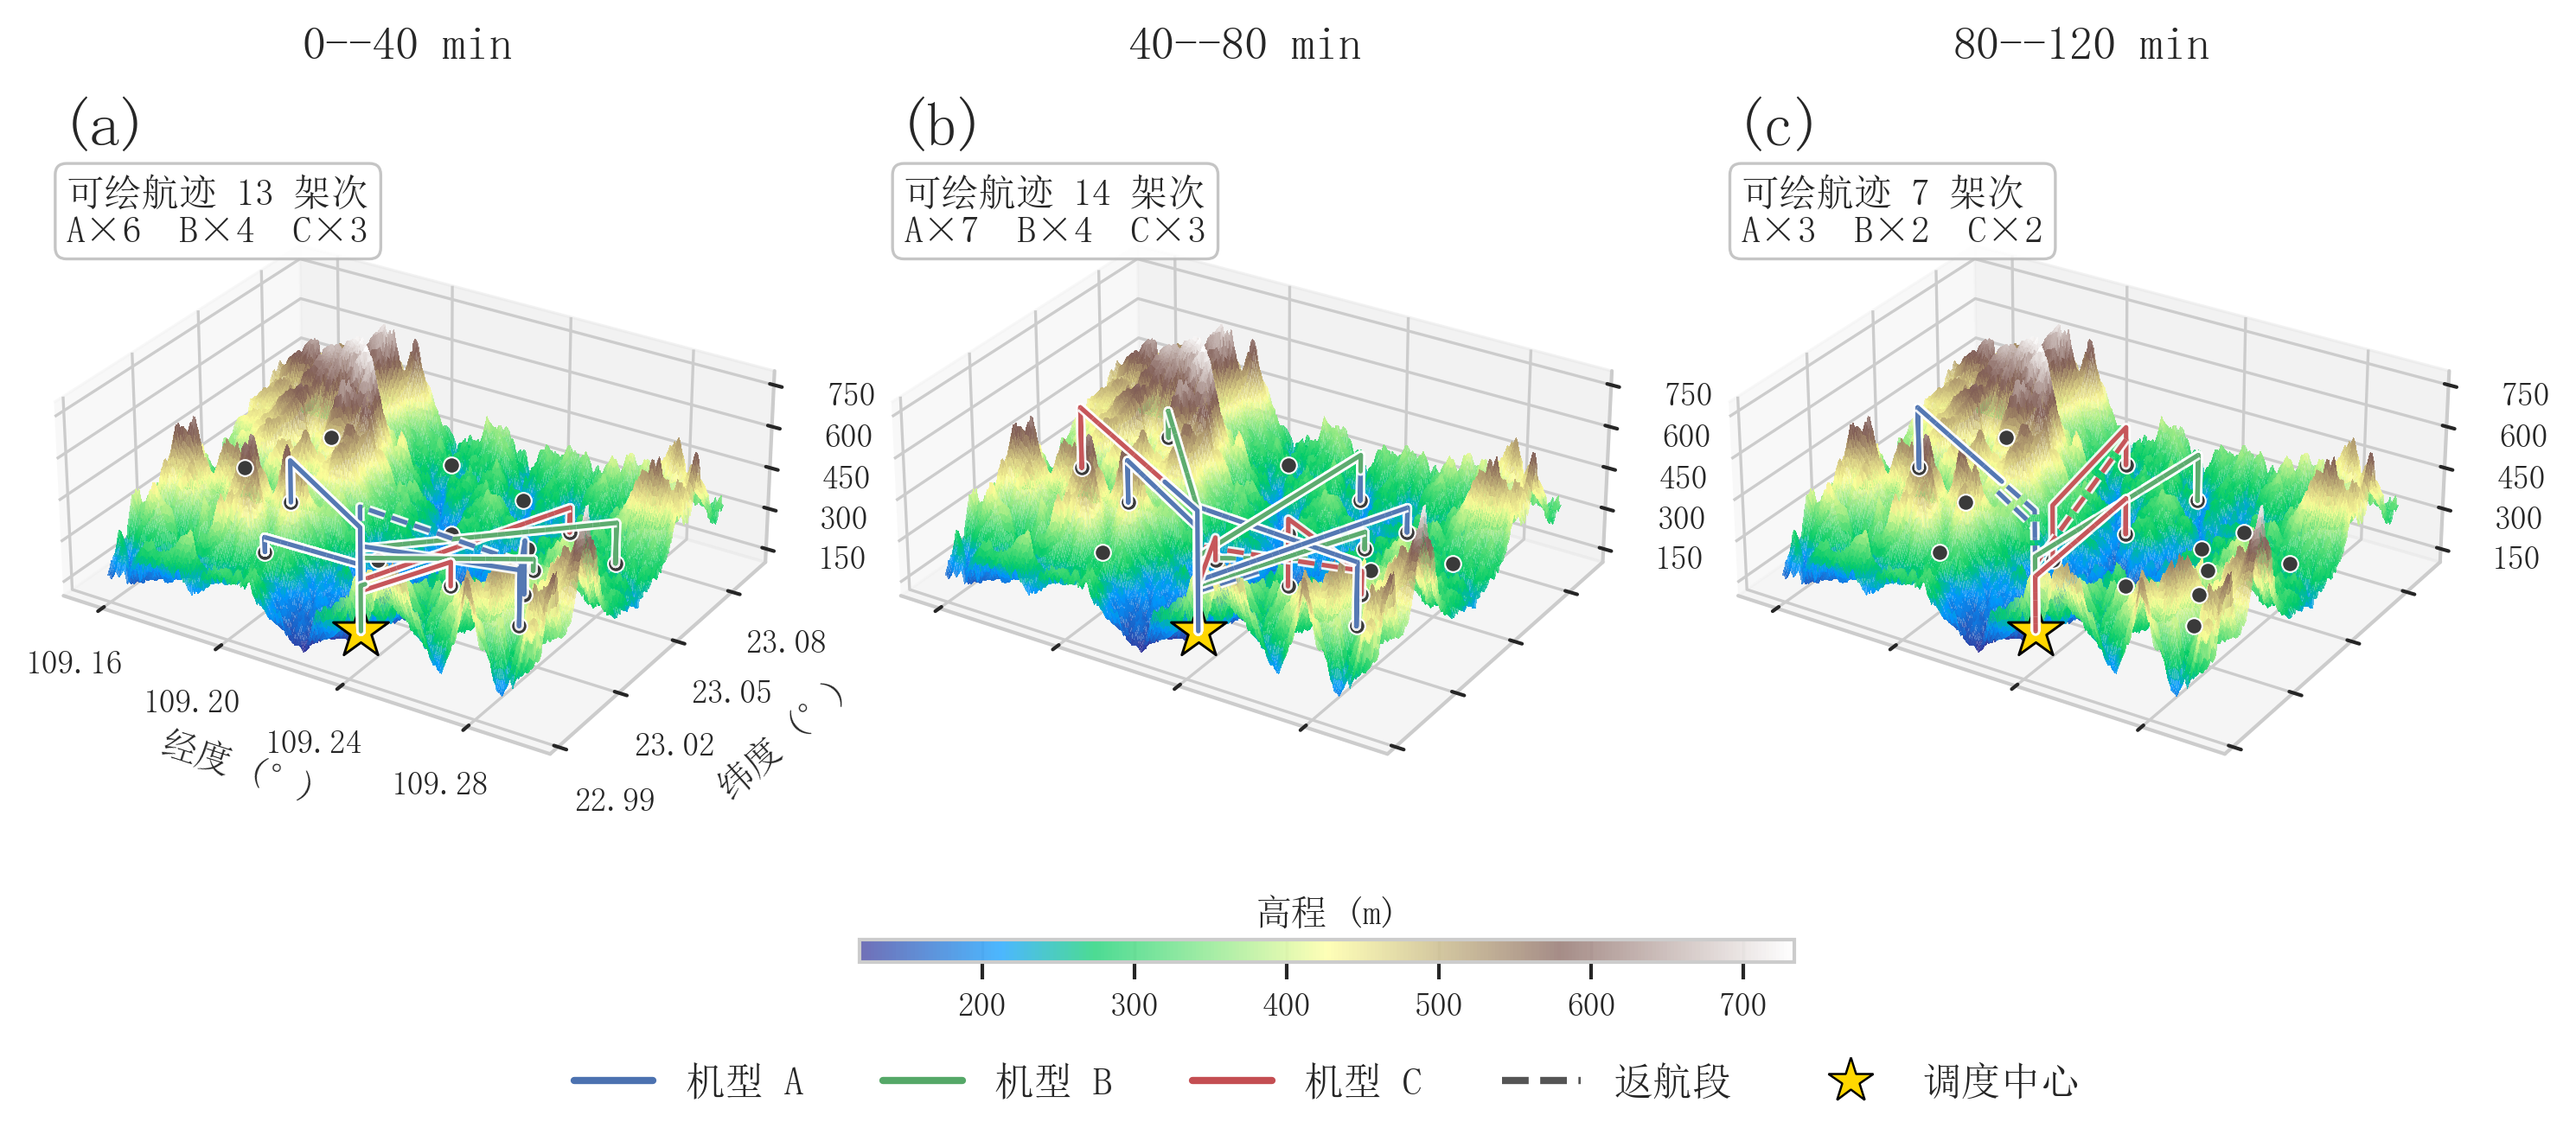
\includegraphics[width=0.95\textwidth]{figures/fig_q2_traj_evolution.png}
	\caption{问题二运输轨迹的分时段演化}
	\label{fig:q2-traj}
\end{figure}

图~\ref{fig:q2-traj}把同样这 24 个架次按 0--40、40--80、80--120\,min 三段切开，各段的航迹叠在同一片三维地形之上：颜色对应机型，实线为投送段、同色虚线为投送完成后的返航段，金色星标是调度中心。三个时段中能画出航迹的架次依次为 13、14、7，三者之和大于 24，是因为单个架次的耗时跨越 40\,min 的分段边界时会被相邻两段各记一次；首段是 13 而非 16，是因为 T14、T15、T16 虽在 40\,min 之前已开始地面准备，其在首段内仍处地面、不足两个采样点，爬升与巡航都落在第二段——图上取的是「该段内确有航迹可画」这一口径，与图中所见一致。第三段只剩 7 条航迹，而其中最后一个返航时刻正是 $6506.1$\,s 的完工时刻（$108.4$\,min）：本方案的收尾阶段在飞机队已相当稀疏，完工时刻落在跨区 C 型架次 T21（S011$\to$S008）的返航上；这与 6.2 节的判断一致——按能耗最小选型会把完工时刻压到只占机队四分之一的 C 型机上，派工优先级 $\pi$ 正是为化解这一瓶颈而引入的。最后是读数口径：纵轴作了约 $7.8$ 倍的垂向夸张（水平实距约 $14.2$\,km $\times$ $10.9$\,km，而窗口内高程幅度不足 $0.9$\,km），故图中的陡缓不能按视觉斜率判读；水平两轴为真实经纬度，服务区点位按其作业海拔（地面以上 30\,m）绘制。
\begin{table}[htbp]
	\caption{问题二的 $\varepsilon$-约束扫描结果}
	\label{tab:q2-pareto}
	\centering
	\small
	\setlength{\tabcolsep}{4.5pt}
	\begin{tabular}{ccccccc}
		\toprule
		架次上限 $K$ & 实际架次 & 能耗（kWh） & 完成时间（h） & 加权时延 & 硬违约 & 非支配 \\
		\midrule
		20 & 20 & 67.033 & 2.53 & 0 & 0 & 是 \\
		22 & 22 & 69.341 & 1.91 & 0 & 0 & 是 \\
		\textbf{25} & \textbf{24} & \textbf{69.316} & \textbf{1.81} & \textbf{0} & \textbf{0} & \textbf{是} \\
		30 & 24 & 69.342 & 1.81 & 0 & 0 & 否 \\
		\bottomrule
	\end{tabular}
\end{table}

表~\ref{tab:q2-pareto}的最右一列按（实际架次、能耗、完成时间、加权时延）四个维度对四档两两比较后逐档标出：只有 $K\le30$ 一档被支配——它与 $K\le25$ 一档的实际架次相同（均为 24 架）、完成时间也相同（$6506.1$\,s），而能耗更高（69.342 对 69.316\,kWh），故被 $K\le25$ 一档严格占优，本文不把它列为前沿档。其余三档互不支配，共同构成四维非支配前沿；四个档位的硬违约均为 $0$。需要说明的是，扫描本身仍然如实保留被支配档的原始记录（\texttt{results/q2\_scan.csv}），标“否”只表示它不进入前沿，不表示该档不可行。

前沿上呈现出一个方向明确但代价不菲的权衡：把架次上限从 20 放宽到 25，完成时间由 $9114.4$\,s 缩至 $6506.1$\,s（$-28.6\%$），代价是架次由 20 增至 24（$+20\%$）、能耗由 67.033 增至 69.316\,kWh（$+3.4\%$）。值得注意的是 $K\le20$ 一档的位置：它是四档中\textbf{能耗最低}（$67.033$\,kWh，比推荐档低 $3.3\%$）、\textbf{架次最少}（20 个）的一档，但完成时间最长（$9114.4$\,s，比推荐档长 $40.1\%$）。三档的加权时延都已为 $0$，无法再靠放宽架次换取。按式~\eqref{eq:q2-key} 的字典序，四档的加权时延并列于 $0$，比较进入第二层「完成时间」，$K\le25$ 档胜出；\textbf{若把能耗置于完成时间之前，则会选中 $K\le20$ 档}。本文取前者，因为题目把「及时性」排在能耗之前，而完成时间是本文口径下对及时性最直接的度量；这一取舍的依据是题目次序，不是「$K\le25$ 档全面更优」——它在能耗与架次上都劣于 $K\le20$ 档。

\textbf{消融实验。}由于派工顺序本身就能带来可观改进，若不做消融，很容易把“顺序的功劳”误记到“组批搜索”头上。故本文固定同一初始解与同一迭代预算（$3\,000$ 轮、单种子），分别关闭顺序搜索与组批搜索；第五行保持与④完全相同的协议（同轮数、同种子、同样放开架次数上限），只把求解引擎换成 6.2 节的三层移植实现，用来把“替换算法”的收益与“打开某个开关”的收益分开。结果如表~\ref{tab:q2-ablation}所示。

\begin{table}[htbp]
	\caption{ALNS 消融实验}
	\label{tab:q2-ablation}
	\centering
	\small
	\begin{tabular}{lccccc}
		\toprule
		配置 & 架次数 & 能耗（kWh） & 完成时间（s） & 加权时延 & 硬违约 \\
		\midrule
		① 基线（FFD 组批 + 紧迫度派工） & 25 & 84.779 & 14\,367.2 & 743\,943 & 0 \\
		② 仅顺序（组批冻结） & 25 & 78.293 & 9\,790.4 & 29\,526 & 0 \\
		③ ALNS（派工顺序固定） & 26 & 73.526 & 7\,235.7 & 0 & 0 \\
		④ ALNS 全量（组批 + 顺序） & 32 & 89.394 & 9\,447.7 & 51\,008 & 0 \\
		⑤ 三层全移（v2 引擎） & 28 & 82.042 & 7\,376.4 & 7\,245 & 0 \\
		\bottomrule
	\end{tabular}
\end{table}

由表~\ref{tab:q2-ablation}可得三点：其一，仅调整派工顺序（②）就把完成时间从 $14\,367.2$\,s 压到 $9\,790.4$\,s（$-31.9\%$）、加权时延降低 $96.0\%$（$743\,943\to29\,526$），说明顺序确实是本题的一等决策变量；其二，进一步开放组批搜索（③）把完成时间压到 $7\,235.7$\,s、能耗降到 $73.526$\,kWh、加权时延归零，是四个“受限配置”中最好的一行；其三，\textbf{④ 与 ⑤ 在放开架次数上限后同时退化}——④ 升到 32 架次、$89.394$\,kWh（比基线高 $5.4\%$）、时延 $51\,008$，⑤ 升到 28 架次、$82.042$\,kWh、时延 $7\,245$，两行的四项指标都不如架次受限的 ③，尽管它们的解空间严格更大。这不是模型矛盾，而是固定迭代预算下的搜索质量问题：推荐解（24 架次、$6506.1$\,s）要求先把架次数压下来，而放开上限后搜索更容易停在“多架次、长完工”的局部解。\textbf{⑤ 对 ④ 的四项全面改进}（架次 28 对 32、能耗 82.042 对 89.394\,kWh、完成时间 $7\,376.4$ 对 $9\,447.7$\,s、时延 $7\,245$ 对 $51\,008$）说明三层移植本身确实有效，只是不足以弥补放开上限带来的退化。本文如实报告这一现象，不将其粉饰为“全量搜索更优”。

推荐方案取 $\varepsilon$-约束扫描中 $K\le25$ 档的可行解（24 架次、69.316\,kWh、$6506.1$\,s、加权时延 0）。把它与消融五行逐维比较：它在\textbf{架次数}（24 对 25 / 25 / 26 / 32 / 28）、\textbf{能耗}（69.316 对 84.779 / 78.293 / 73.526 / 89.394 / 82.042\,kWh）、\textbf{完成时间}（$6506.1$ 对 $14\,367.2$ / $9\,790.4$ / $7\,235.7$ / $9\,447.7$ / $7\,376.4$\,s）与\textbf{加权时延}（0 对 $743\,943$ / $29\,526$ / 0 / $51\,008$ / $7\,245$）四项上\textbf{均不差且至少一项严格更优}，即对全部五个配置构成\textbf{全面占优}。但这一比较的边界必须讲清楚：消融各行统一取 $3\,000$ 轮、单种子、同一初始解，而推荐解来自 $5$ 种子 $\times$ $3\,500$ 轮 $\times$ $4$ 档的扫描再加逐档定型，预算远大于消融各行。故它说明的是“\textbf{本文的完整求解链优于任一单项配置}”，\textbf{不能}读作“算法在同等预算下全面更优”。

\subsection{小规模精确验证}

ALNS 是启发式，其解的质量需要独立证据。本文设计两层小规模精确验证，验证逻辑与适用范围均如实标注。

\textbf{Layer A（分区层，无路径简化）。}取 3 个服务区构成小算例，穷举全部架次模式（列生成）后用两层字典序集合划分整数规划求精确最优：先最小化架次数，再在最小架次下最小化能耗。这里必须说明正确性的理由不是“架次最多访问 3 个服务区”——该命题为假，实测存在能量可行的 5 服务区架次——而是：算例只含 3 个服务区时，任何架次的区域集合必然是该 3 区的子集，故 3 个区的 6 个排列即全部可能路径，区域集合与访问顺序被同时穷举。为保证对比有效，ALNS 在该算例上以同一服务区子集运行。

\begin{table}[htbp]
	\caption{ALNS 与精确解的最优性间隙}
	\label{tab:q2-exact}
	\centering
	\footnotesize
	\setlength{\tabcolsep}{4pt}
	\begin{tabular}{llcccc}
		\toprule
		层级 & 算例 & 模型规模 & 精确模型 & 启发式对照 & 精确相对启发式 \\
		\midrule
		A & S013+S014+S015（9 箱） & 160 列 & 2 架次 / 7.3226 & ALNS 2 / 7.3226 & $0$ \\
		A & S009+S010+S011（9 箱） & 1\,068 列 & 2 架次 / 6.3665 & ALNS 2 / 6.3665 & $0$ \\
		A & S002+S009+S010（14 箱） & 6\,262 列 & 3 架次 / 12.9433 & ALNS 3 / 12.9433 & $0$ \\
		\addlinespace
		B1 & 固定指派·最短完工 & 118 二元 & 14\,029.8\,s\dag & 贪心 14\,367.2\,s & $+2.40\%$ \\
		B1$'$ & 固定指派·加权时延 & 118 二元 & 703\,470.6\ddag & 贪心 743\,943.2 & $+5.75\%$ \\
		B2 & 自由指派·最短完工 & 630 二元 & 13\,565.2\,s\S & 贪心 14\,367.2\,s & 见注~\S \\
		\bottomrule
	\end{tabular}

	\vspace{2pt}
	{\footnotesize \dag\ 已证最优，但该解\textbf{违反 8 项硬时限}，只作下界参考；\quad
	\ddag\ 已证最优，加权时延口径，硬违约 $0$；\quad
	\S\ 90\,s 时限内\textbf{未证最优}（上下界间隙 $65.77\%$），此为该时刻的可行上界；该上界虽比贪心排程\textbf{短 $5.58\%$}，但它\textbf{违反 9 项硬时限}，不构成可行方案，故该行不给出“精确相对启发式”的比值。}
\end{table}

Layer A 的三个算例最优性间隙全部为 $0$，且都在 1\,000 次迭代内收敛。值得强调的是，这层验证并非装饰：最初的 ALNS 在三个算例上跨 3 个随机种子、12\,000 次迭代都\textbf{系统性停在 3 架次}（非最优），排查后确认根因正是上文所述的代理代价缺陷——B 型无人机仅 2 架，而最优解需要“把 S013 与 S014 合并为一架 C 型架次以腾出一架 B 给 S015”，该动作在代理代价下永远显示为“更贵”。补入成组修复算子后间隙归零。这正是“小规模精确解验证启发式”的实际价值：它抓到了一个贪心代理看不见的机队瓶颈型协同。

\textbf{适用范围必须声明}：Layer A 的三个算例均只含 3 个服务区，8 架无人机对至多 9 个架次，\textbf{机队资源竞争几乎不存在}，故它验证的是组批、能耗与路径逻辑的正确性，\textbf{不能}外推为“全局资源拥塞情形下已证最优”。

\textbf{Layer B（时序层，big-M 析取 MILP）。}固定贪心方案的机型指派，只放开架次的执行无人机、共享电池与开始时刻，用 big-M 析取约束表达“同一无人机/电池的占用区间不重叠”\cite{grossmann2011generalized}。$M$ 的取值必须满足 $M\ge UB+\max\tau$（$\max\tau$ 为全部充电操作中最长的充电时长；此处不引入充电资源的下标，以免与货箱编号 $c$ 撞车），其中 $UB$ 由一份\textbf{计入充电占用的完全串行排程}给出（本文实测：取 $M=UB$ 会漏掉充电等待而制造假不可行，这个坑踩过）；为保证该界不截掉可行解，还对贪心排程本身做了暖可行性回放，实测 $M=94\,881.2$\,s、贪心完工距上界尚有 $80\,514$\,s 余量。两个固定指派变体分别以最短完工与最小加权时延为目标，分别在 3.4\,s 与 2.3\,s 内证到最优（均含列与约束构建时间），且解回放后无资源重叠。第三行的自由指派变体在 90\,s 时限内\textbf{未证到最优}，本文按实测状态如实记为“超时但有可行解”，不记为不可行、也不记为最优。

两个层次得到的间隙与劣化幅度并排呈现于图~\ref{fig:q2-exact}。

\begin{figure}[htbp]
	\centering
	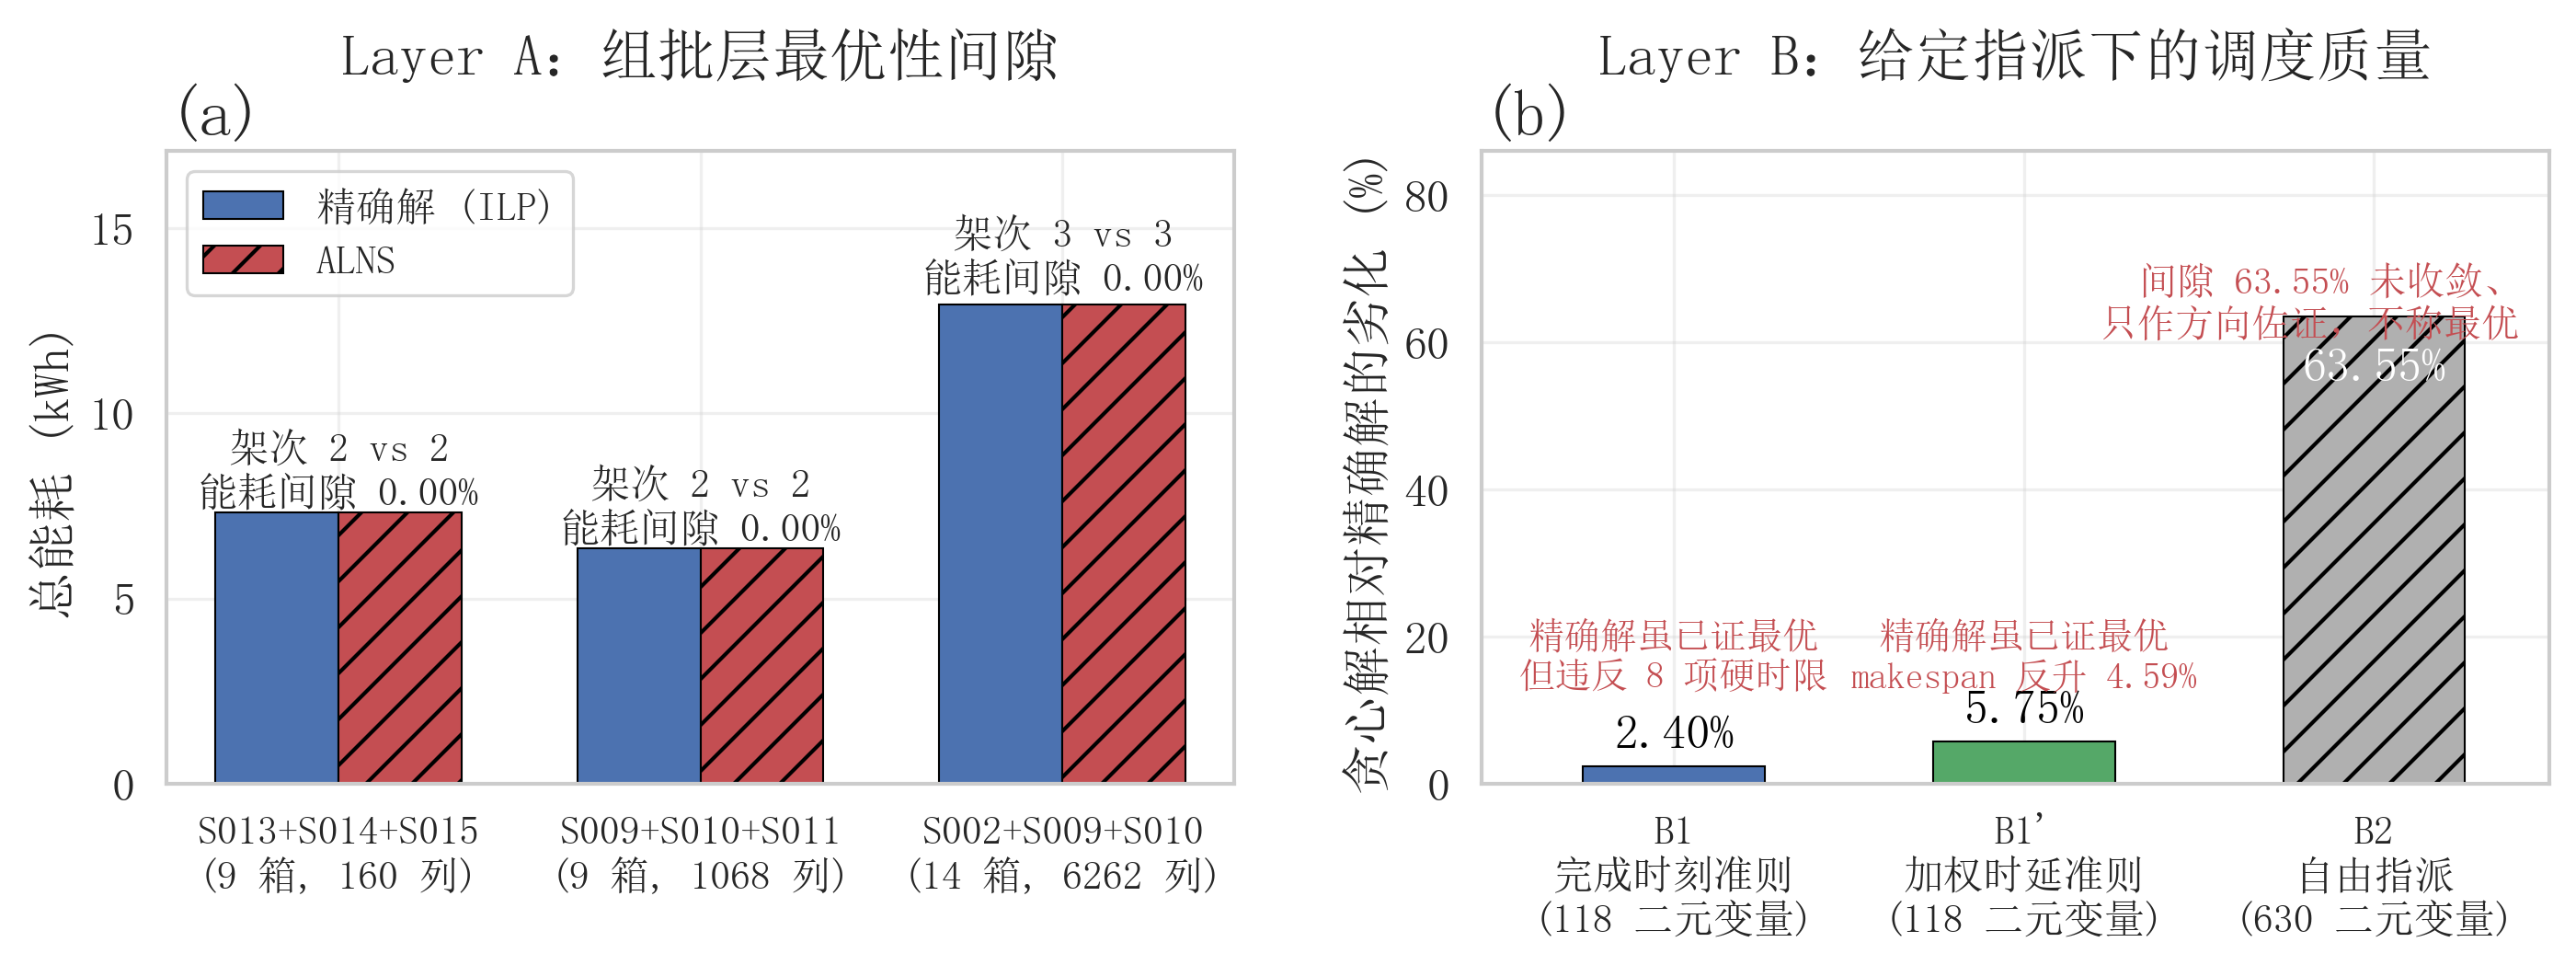
\includegraphics[width=0.95\textwidth]{figures/fig_q2_exact.png}
	\caption{ALNS 相对精确解的劣化与间隙}
	\label{fig:q2-exact}
\end{figure}

图~\ref{fig:q2-exact}把表~\ref{tab:q2-exact}的间隙按口径并排呈现。B1 与 B1$'$ 给出的是“给定贪心指派，贪心调度已接近最优”的\textbf{证书}：最短完工口径下贪心仅比最优差 $2.40\%$（$14\,367.2$ 对 $14\,029.8$\,s），加权时延口径下仅差 $5.75\%$（$743\,943.2$ 对 $703\,470.6$）；而两者互相印证了“完成时间与时延不可兼得”——B1 的最优解 makespan 最短，但其\textbf{违反 8 项硬时限}（故不作为可行方案，仅作下界参考）；B1$'$ 的最优解硬违约数为 0，但其 makespan 为 15\,026.7\,s，比贪心还差 $4.59\%$。B2 放开了物理指派，变量数由 118 增至 630，求解 90\,s 后上下界间隙仍有 $65.77\%$。该时刻的可行上界为 13\,565.2\,s，比贪心排程（14\,367.2\,s）还短 $5.58\%$——但它\textbf{违反 9 项硬时限}，与 B1 一样只是「放松问题的一个下界方向」，不是可交付的方案；而 65.77\% 的间隙也说明这个上界离真正的最优还差得远。故本文\textbf{不把 B2 计入任何最优性结论}，也不引用其目标值作为对照——它只说明「自由指派层的精确求解规模已超出 90\,s 能处理的范围」，这一局限已列入第 10 章的模型缺点。

最后说明货箱到架次的映射关系。图~\ref{fig:q2-flow}给出推荐方案中“服务区—架次—机型”的三层流向，可以看出流量在 C 型与 B 型之间的分配与问题一的结论一致：重载服务区走 C 型，轻载服务区走 B 型，而 A 型主要承担紧急货箱的轻载快投。

\begin{figure}[htbp]
	\centering
	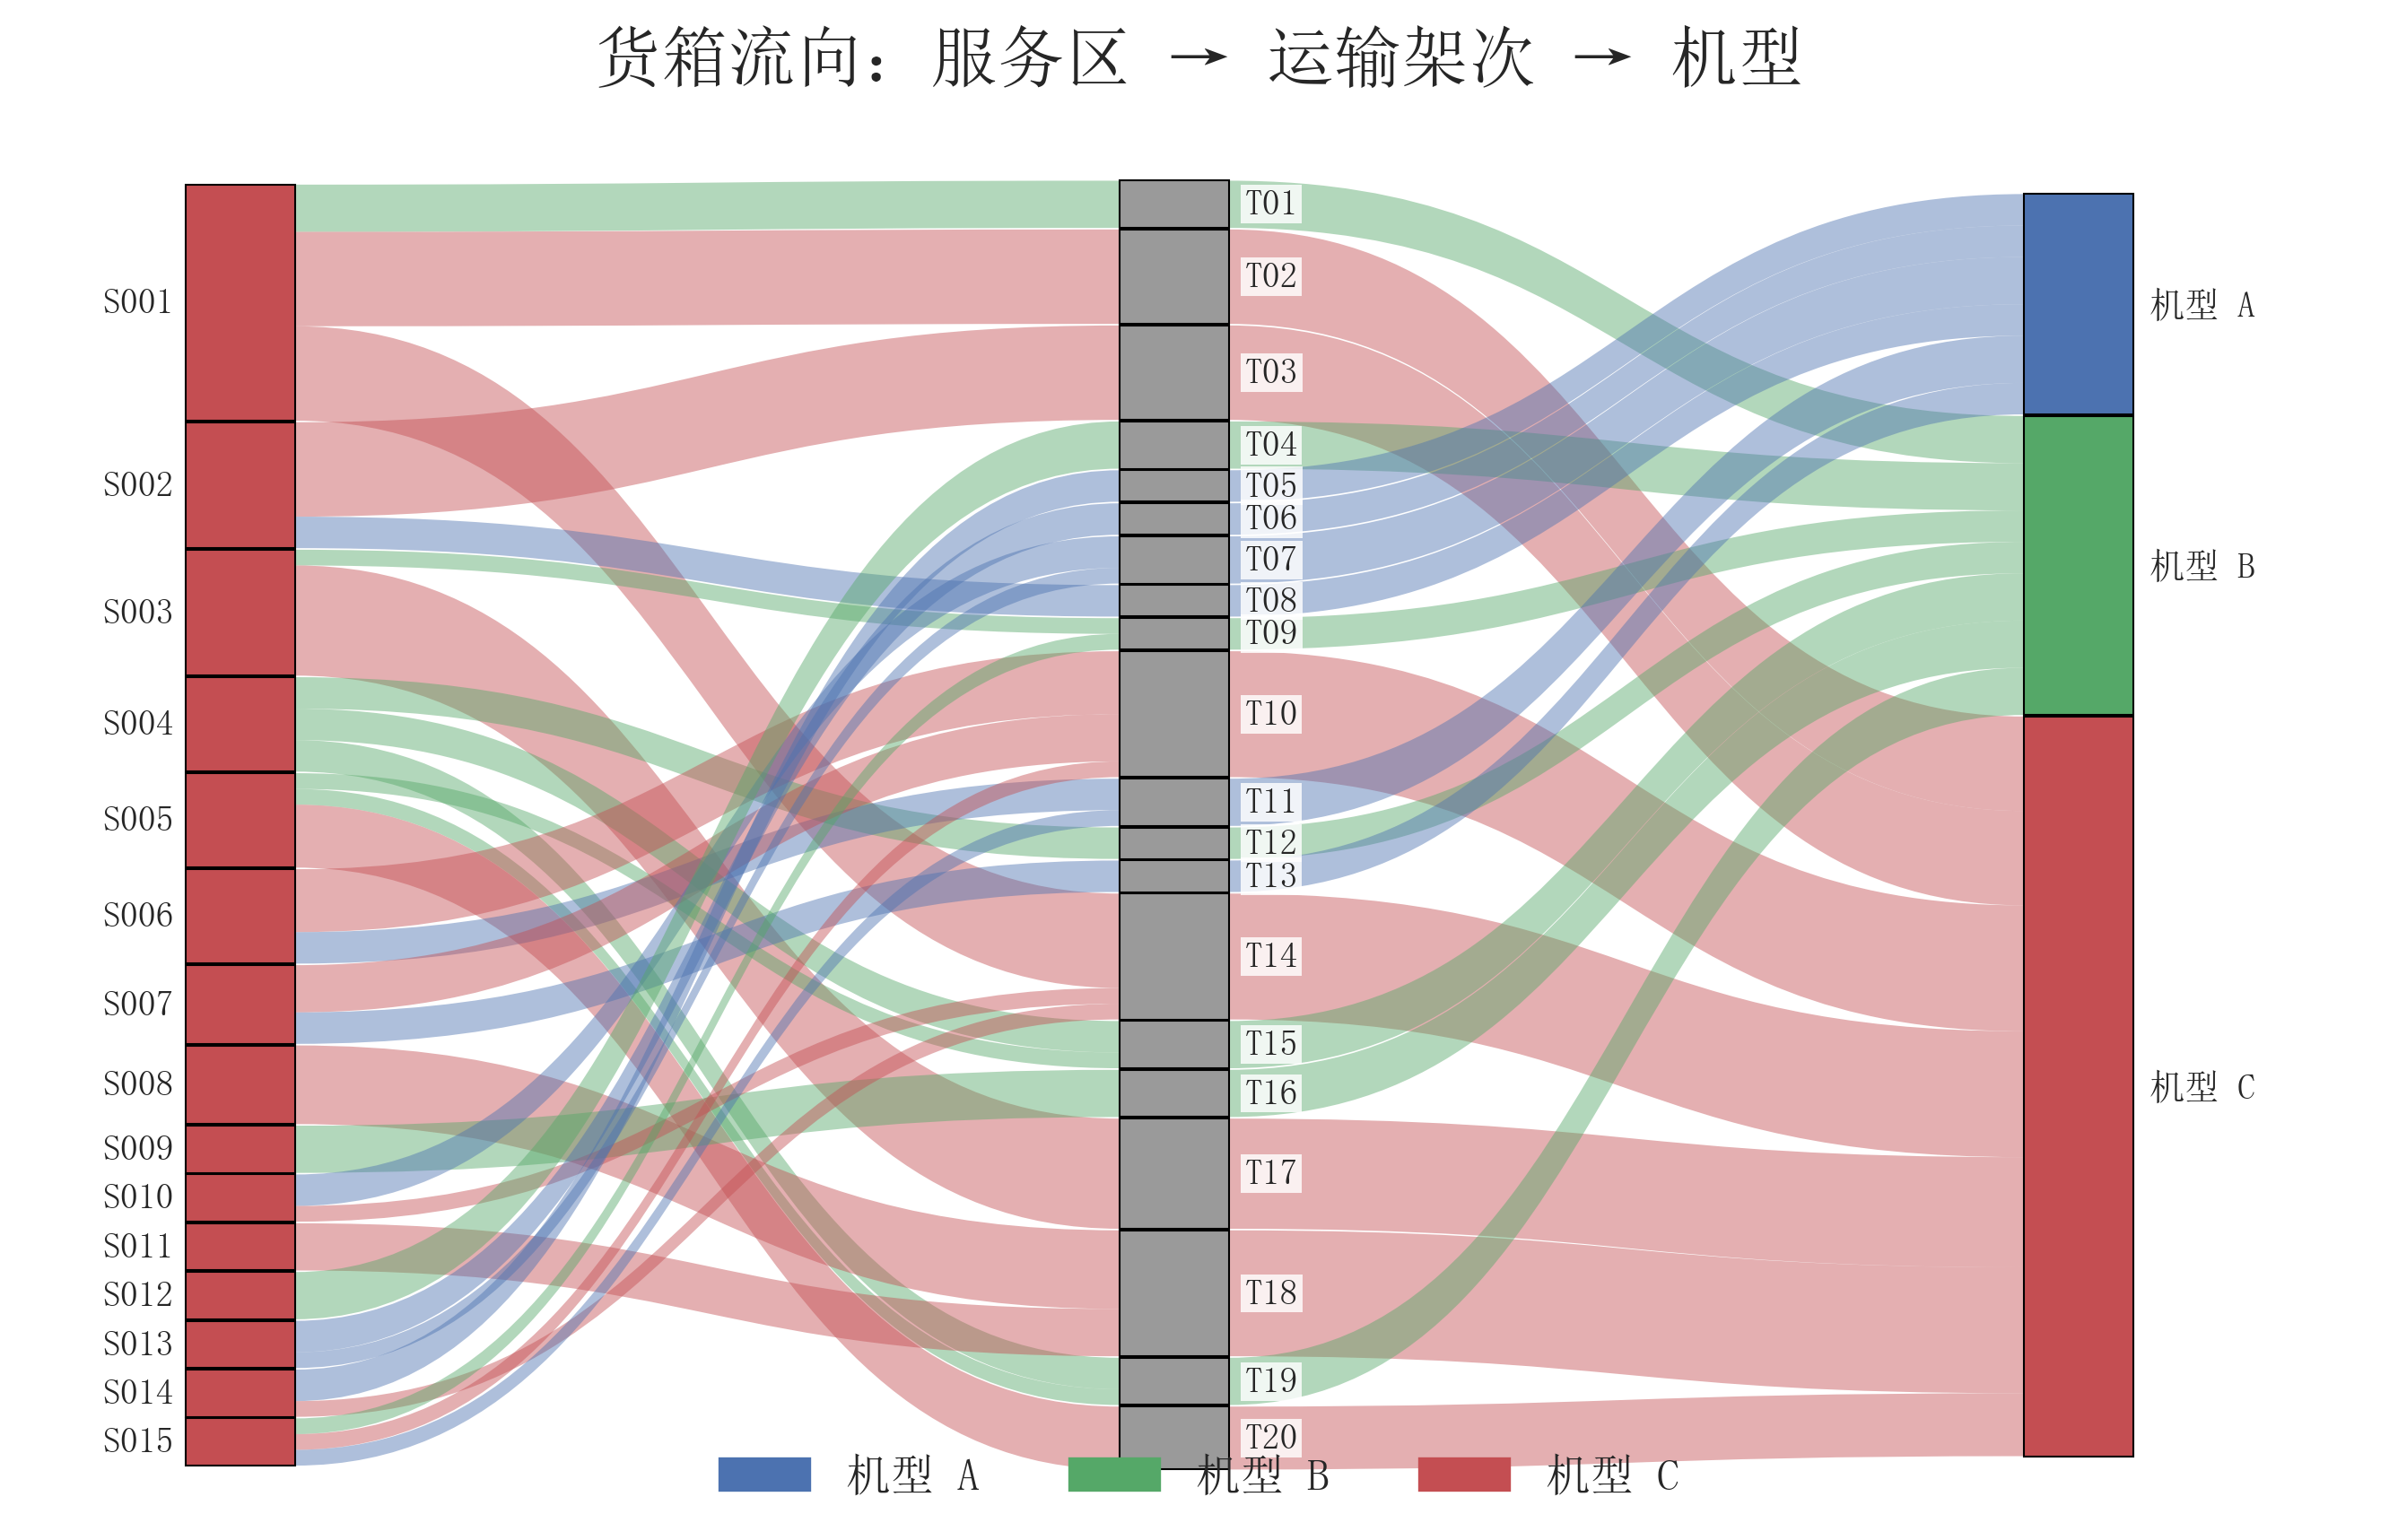
\includegraphics[width=0.95\textwidth]{figures/fig_q2_flow.png}
	\caption{服务区—架次—机型的三层流向}
	\label{fig:q2-flow}
\end{figure}

\textbf{本节向问题三输送什么。}问题二的产出是一张完整的运输时刻表：24 个架次各自的机型、访问顺序与开始时刻，80 个货箱各自的承运架次与交付时刻。问题三直接站在这张表上——它的输入校验要求错峰表 \texttt{q3\_stagger.csv} 的「原开始时刻」一列恒等于问题二架次表的「开始时刻」（第 \ref{sec:feasib-deliv} 节），也就是说不允许下游悄悄换一张时刻表再声称「在问题二基础上改进」。承接的方式则是有选择的：问题三\textbf{保留组批与航线不变}（哪个货箱在哪架次、架次访问哪些服务区都不重排），只把开始时刻当作可调量，再在其上叠加中继侧的决策（悬停站的坐标与离地高度、中继架次的派发与能源组件分配）。这一层切分是本文为控制搜索规模而作的设计选择，不是题目的可行域要求：题目并未禁止相对问题二基线提前，提前是否可行只取决于释放、无人机与电池的就绪时刻以及硬时限。代价则很明确——「靠改组批、改航线或提前腾出通信余量」这部分解空间被放弃了，该局限列入第 10 章。
